\begin{figure}[!ht]
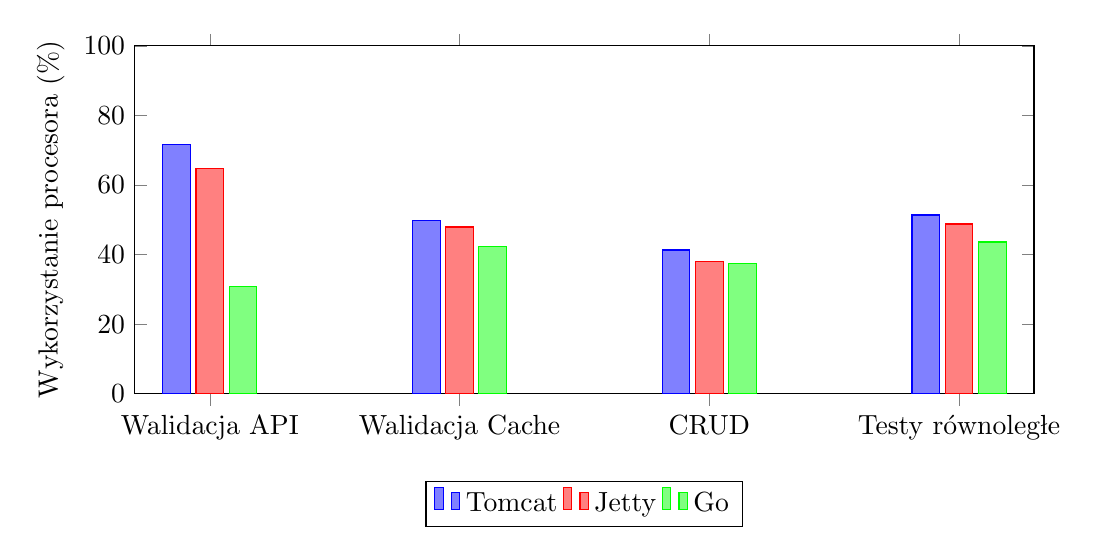
\begin{tikzpicture}
\begin{axis}[
    ybar,
    width=13cm,
    height=6cm,
    legend style={at={(0.5,-0.25)},
      anchor=north,legend columns=-1},
    ylabel={Wykorzystanie procesora (\%)},
     symbolic x coords={Walidacja API, Walidacja Cache, CRUD, Testy równoległe},
    xtick=data,
    ymin=0, ymax=100
    ]
\addplot [blue, fill=blue!50!white] coordinates{ (Walidacja API,71.62) (Walidacja Cache,49.82) (CRUD,41.32) (Testy równoległe,51.37) } ;
\addplot [red, fill=red!50!white] coordinates{ (Walidacja API,64.72) (Walidacja Cache,47.93) (CRUD,37.96) (Testy równoległe,48.79) } ;
\addplot [green, fill=green!50!white] coordinates{ (Walidacja API,30.79) (Walidacja Cache,42.43) (CRUD,37.34) (Testy równoległe,43.62) } ;
\legend{Tomcat,Jetty,Go}
\end{axis}
\end{tikzpicture}
\caption{Wykorzystanie procesowa przez aplikacje podczas testów z pustą bazą danych}
\label{fig:cpu_utilization_clean}
\end{figure}


\begin{figure}[!ht]
\begin{tikzpicture}
\begin{axis}[
    ybar,
    width=13cm,
    height=6cm,
    legend style={at={(0.5,-0.25)},
    anchor=north,legend columns=-1},
    ylabel={Wykorzystanie pamięci RAM (MB)},
    symbolic x coords={Walidacja API, Walidacja Cache, CRUD, Testy równoległe},
    xtick=data,
    ymin=0
]
\addplot [blue, fill=blue!50!white] coordinates{ (Walidacja API,1904.32) (Walidacja Cache,1972.46) (CRUD,1996.97) (Testy równoległe,2020.42) } ;
\addplot [red, fill=red!50!white] coordinates{ (Walidacja API,2012.54) (Walidacja Cache,1900.86) (CRUD,1679.41) (Testy równoległe,1772.25) } ;
\addplot [green, fill=green!50!white] coordinates{ (Walidacja API,220.19) (Walidacja Cache,224.31) (CRUD,232.18) (Testy równoległe,233.85) } ;
\legend{Tomcat,Jetty,Go}
\end{axis}
\end{tikzpicture}
\caption{Wykorzystanie pamięci na serwerze podczas testów z pustą bazą danych}
\label{fig:mem_utilization_clean}
\end{figure}


\begin{figure}[!ht]
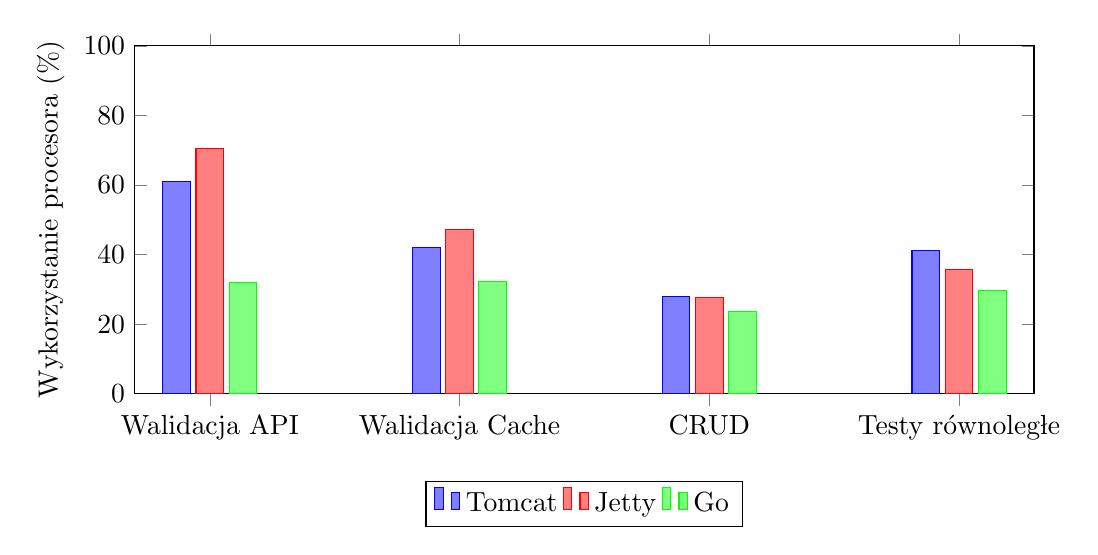
\begin{tikzpicture}
\begin{axis}[
ybar,
width=13cm,
height=6cm,
legend style={at={(0.5,-0.25)},
anchor=north,legend columns=-1},
ylabel={Wykorzystanie procesora (\%)},
symbolic x coords={Walidacja API, Walidacja Cache, CRUD, Testy równoległe},
xtick=data,
ymin=0, ymax=100
]
\addplot [blue, fill=blue!50!white] coordinates{ (Walidacja API,60.97) (Walidacja Cache,42.12) (CRUD,27.96) (Testy równoległe,41.23) } ;
\addplot [red, fill=red!50!white] coordinates{ (Walidacja API,70.38) (Walidacja Cache,47.28) (CRUD,27.77) (Testy równoległe,35.66) } ;
\addplot [green, fill=green!50!white] coordinates{ (Walidacja API,31.87) (Walidacja Cache,32.27) (CRUD,23.57) (Testy równoległe,29.74) } ;
\legend{Tomcat,Jetty,Go}
\end{axis}
\end{tikzpicture}
\caption{Wykorzystanie procesowa na serwerze podczas testów z bazą danych wypełnioną danymi początkowymi}
\label{fig:cpu_utilization_full}
\end{figure}

\begin{figure}[!ht]
\begin{tikzpicture}
\begin{axis}[
ybar,
width=13cm,
height=6cm,
legend style={at={(0.5,-0.25)},
anchor=north,legend columns=-1},
ylabel={Wykorzystanie pamięci RAM (MB)},
symbolic x coords={Walidacja API, Walidacja Cache, CRUD, Testy równoległe},
xtick=data,
ymin=0
]
\addplot [blue, fill=blue!50!white] coordinates{ (Walidacja API,1948.69) (Walidacja Cache,2018.4) (CRUD,1902.79) (Testy równoległe,1852.85) } ;
\addplot [red, fill=red!50!white] coordinates{ (Walidacja API,1985.77) (Walidacja Cache,2050.25) (CRUD,2016.22) (Testy równoległe,2005.91) } ;
\addplot [green, fill=green!50!white] coordinates{ (Walidacja API,245.44) (Walidacja Cache,248.03) (CRUD,256.16) (Testy równoległe,257.09) } ;
\legend{Tomcat,Jetty,Go}
\end{axis}
\end{tikzpicture}
\caption{Wykorzystanie pamięci na serwerze podczas testów z bazą danych wypełnioną danymi początkowymi}
\label{fig:mem_utilization_full}
\end{figure}